\documentclass[a4paper,12pt]{article}
\author{Konrad Simlinger}
\title{GalleryGenie \\
		An Intelligent Image Tagging System}



%Custom Commands
\newcommand{\imgal}{GalleryGenie}
\newcommand{\imgalapp}{\color{client}\imgal App\color{black}}
\newcommand{\imgalclient}{\color{client}\imgal Client\color{black}}
\newcommand{\imgalserver}{\color{server}\imgal Server\color{black}}

\usepackage{amsmath} %notwendig für math
\usepackage{graphicx} %notwendig für .png .jpg .pdf1
\usepackage{multicol} %notwendig für multiple columns
\usepackage{soul} %striketrough


\usepackage{fontspec-luatex}
\usepackage{fontspec}

\usepackage{xcolor}
\usepackage{titlesec}

\setmainfont{Spectral Light}
\setsansfont{Comfortaa}
\setmonofont{JetBrainsMono Nerd Font}


\definecolor{client}{rgb}{0.4,0,1}
\definecolor{server}{rgb}{0.75,0,0.4}

\begin{document}
%\sffamily % SANS SERIF
\maketitle
\newpage
\tableofcontents
\newpage

\section{Description}
\textbf{\imgal{}} is an intuitive and intelligent image organization and management application that streamlines the process of managing large collections of digital images. The application offers an easy-to-use and visually appealing interface for storing, categorizing, and searching for images.  \st{With its advanced image analysis algorithms, GalleryGenie automatically generates tags for each uploaded image, which helps users to easily search for and find specific images}. Additionally, when a new image is uploaded, the application compares it to the images already stored in the gallery and identifies any similarities using a sophisticated likeness scoring algorithm. If a high likeness score is detected, the user is prompted to automatically copy some or all of the tags from the compared image, saving the user time and effort. With features like automatic tagging and similarity detection, \imgal{} is the perfect tool for anyone looking to efficiently manage their digital image collections.

\newpage
\section{Database}
\subsection{Database Design}

\begin{table}[h]
	\begin{tabular}{ll}
		\multicolumn{2}{c}{u\_users}                   \\ \hline
		\multicolumn{1}{l|}{u\_id}           & INT PK     \\
		\multicolumn{1}{l|}{u\_name}         & VARCHAR \\
		\multicolumn{1}{l|}{u\_creationdate} & DATE   
	\end{tabular}
\end{table}

\begin{table}[h]
	\begin{tabular}{ll}
		\multicolumn{2}{c}{p\_pools}           \\ \hline
		\multicolumn{1}{l|}{p\_id}   & INT PK     \\
		\multicolumn{1}{l|}{u\_name} & VARCHAR
	\end{tabular}
\end{table}

\begin{table}[h]
	\begin{tabular}{ll}
		\multicolumn{2}{c}{p\_posts}                   \\ \hline
		\multicolumn{1}{l|}{p\_id}           & INT PK  \\
		\multicolumn{1}{l|}{p\_title}        & VARCHAR \\
		\multicolumn{1}{l|}{p\_u\_author}    & INT FK  \\
		\multicolumn{1}{l|}{p\_p\_pool}      & INT FK  \\
		\multicolumn{1}{l|}{p\_creationdate} & DATE   
	\end{tabular}
\end{table}

\begin{table}[!h]
	\begin{tabular}{ll}
		\multicolumn{2}{c}{pt\_posttags}           \\ \hline
		\multicolumn{1}{l|}{pt\_p\_id} & INT PK FK \\
		\multicolumn{1}{l|}{pt\_t\_id} & INT PK FK
	\end{tabular}
\end{table}

\begin{table}[!h]
	\begin{tabular}{ll}
		\multicolumn{2}{c}{t\_tags}                  \\ \hline
		\multicolumn{1}{l|}{t\_id}         & INT PK  \\
		\multicolumn{1}{l|}{t\_name}       & VARCHAR \\
		\multicolumn{1}{l|}{t\_t\_implies} & INT FK 
	\end{tabular}
\end{table}

\newpage
\subsubsection{EER-Model}
\begin{figure}[!ht]
	%\centering
	\includegraphics[height=300px]{../imgs/EER-Modell-V1.png}
\end{figure}

\newpage
\subsection{Database Development Methodology}
I chose to use the code-first database development methodology for my project because it allows me to quickly and easily develop and iterate on my database schema directly within my application code. With code-first development, I can define my data model in a simple, declarative syntax using C\# classes and annotations, rather than having to manually create tables and columns using SQL scripts or external database management tools.

This approach has several advantages. First, it makes it much faster and easier to develop my database schema, as I can simply define it alongside the rest of my application code, without having to switch back and forth between different tools or languages. Additionally, by using C\# classes to define my data model, I can take advantage of the full range of object-oriented programming techniques, such as inheritance, encapsulation, and abstraction, to create a more modular and maintainable schema.

Another major advantage of code-first development is that it allows me to easily integrate my database development process with my overall software development workflow. By defining my data model directly in code, I can use the same version control tools and development processes that I use for the rest of my application code, making it easier to manage changes and track issues.

Overall, the code-first approach allows me to rapidly develop and iterate on my database schema, while also integrating it more seamlessly with the rest of my application code. By enabling me to take full advantage of object-oriented programming techniques and to use the same development tools and processes for my data model as for the rest of my code, code-first development is a powerful and flexible methodology that is well-suited to my project's needs.

\newpage
\section{User Interface}
The user interface of my application is designed to be intuitive and user-friendly. Each screen is carefully crafted to provide the user with the information and controls they need to easily manage and organize their images. The user interface will feature a clean and modern design, with a focus on simplicity and ease-of-use. It also incorporates a range of interactive features, such as drag-and-drop image uploading and automatic tag suggestions, to make the user experience as smooth and efficient as possible.
\subsection{Prototyping}
\subsubsection{Login Screen}

\begin{figure}[!h]
	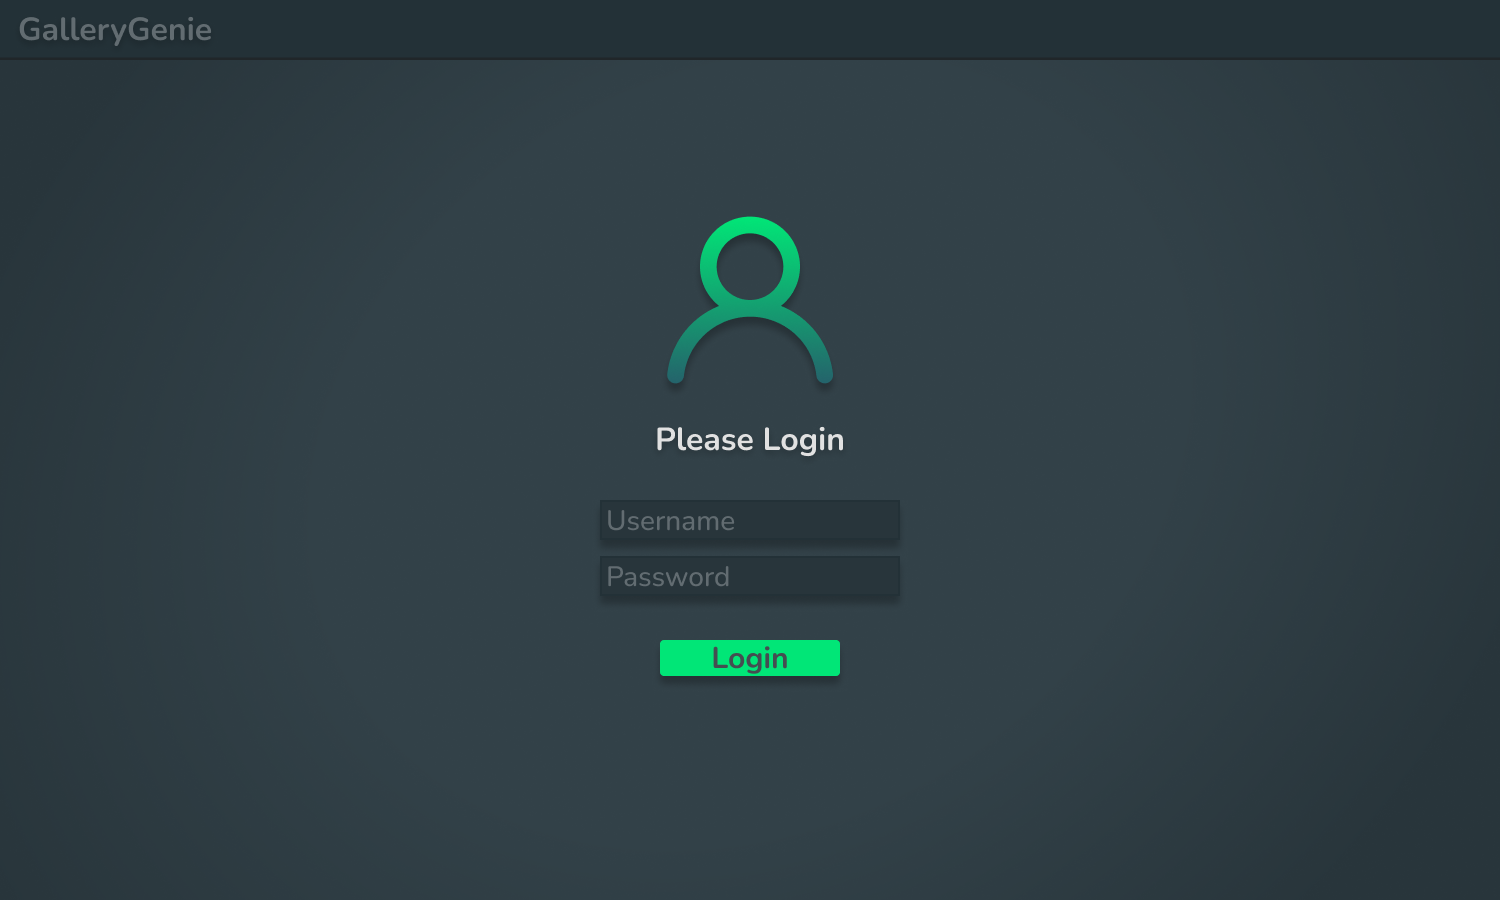
\includegraphics[width=\linewidth]{../imgs/Login.png}
\end{figure}

\newpage
\subsection{Colour Palletes}
\begin{figure}[!h]
	\includegraphics[width=\linewidth,height=\columnwidth]{../imgs/Colours.png}
\end{figure}

\newpage
\subsection{Structure}


\section{Code Architecture}
\subsection{Structure}
The Project is strictly divided into two parts. The \imgalapp{}  and \imgalserver{}. Currently the idea is that the former does not need a live server to function. But instead the Server is an addition to the client. Although the WPF-App is capable of saving and managing the images on its own, it can be used in unison with the \imgalserver{} which functions in a very simple way.


\subsection{\imgalapp}

\subsection{\imgalserver}
The \textbf{\imgalserver{}} is a plain \textbf{.NET} Application that listens for connection from a \imgalclient{}. Once a client connects to the Server over the internet, every action that is taken on the client gets rerouted to the server instead of being saved and executed in the local storage.
\subsection{Developer Notes}
Because this project is designed to be done in and for school, I really don't expect to finish the \imgalapp{} and the \imgalserver{}. Mostly because I overshot my own capabilities and free time. So the main priority of the project lingers on the WPF-App.


\end{document}
